\documentclass[british]{article}
\usepackage[T1]{fontenc}
\usepackage[latin9]{inputenc}
\usepackage{geometry}
\geometry{verbose,tmargin=3.5cm,bmargin=3.5cm,lmargin=3cm,rmargin=3cm}
\usepackage{array}
%\usepackage{multirow}
\usepackage{amstext}
\usepackage{graphicx}
\usepackage{color}
\usepackage[font=small,labelfont=bf]{caption}
%\usepackage{subfigure}

\newcommand{\tabincell}[2]{\begin{tabular}{@{}#1@{}}#2\end{tabular}}

\newcommand{\mytablefontsize}{7pt}
\newcommand{\mytablebaselineskip}{0.7}
\newcommand{\mytabcolsep}{3pt}

\newcommand{\medianInterval}[1]{}

\makeatletter

\newif\iftest
\testfalse

\newif\ifruntime
\runtimefalse

\newif\ifablation
\ablationfalse

\newif\iffeatures
\featuresfalse

%%%%%%%%%%%%%%%%%%%%%%%%%%%%%% LyX specific LaTeX commands.
%% Because html converters don't know tabularnewline
\providecommand{\tabularnewline}{\\}

%%%%%%%%%%%%%%%%%%%%%%%%%%%%%% User specified LaTeX commands.

\title{Configuration Report for the Solver SCIP on the Training Instance Set Europe\textunderscore 3h\textunderscore year \iftest and Testing Instance Set @@instanceSetTest@@ \fi in \emph{Sparkle} }
\author{ Automatically generated by \emph{Sparkle} (version: 0.9.3.2) }

\makeatother

\usepackage{babel}
\begin{document}
\maketitle %


\section{Introduction}
\label{sec:Introduction}

\emph{Sparkle} \cite{Hoos15} is a multi-agent problem-solving platform based on Programming by Optimisation (PbO) \cite{Hoos12}, and provides a number of effective algorithm optimisation techniques (such as automated algorithm configuration, portfolio-based algorithm selection, etc) to accelerate existing solvers.

This experimental report is automatically generated by \emph{Sparkle}. This report presents experimental results on the scenario of configuring the solver SCIP on the training instance set Europe\textunderscore 3h\textunderscore year\iftest~and evaluating it on the testing instance set @@instanceSetTest@@\fi.


\section{Information about the Instance Set(s)}

\begin{itemize}
\item Training set: \textbf{Europe\textunderscore 3h\textunderscore year}, consisting of 12 instances
\iftest\item \textbf{@@instanceSetTest@@}, consisting of @@numInstanceInTestingInstanceSet@@ instances\fi
\end{itemize}


\iffeatures
    \section{Feature Extractors}
        There are @@numFeatureExtractors@@ feature extractor(s) included in \emph{Sparkle}, as listed below.

        \begin{enumerate}
        @@featureExtractorList@@
        \end{enumerate}

        \emph{Sparkle} uses all the feature extractors presented above to compute a feature vector for each training instance. Every feature extractor computes a feature vector for each training instance. The final feature vector is then the combination of all computed feature vectors. The cutoff time for feature vector computation on each training instance is set to @@featureComputationCutoffTime@@ seconds. This time is shared equally between the feature extractors.

        The calculated instance features are then passed on to be used in the process of solver configuration. 

\fi


\section{Information about the Configuration Protocol}

The configurator used by \emph{Sparkle} in this scenario is SMAC2 ({\em Sequential Model-based Algorithm Configuration}) \cite{SMAC2}, and the version of SMAC2 used in \emph{Sparkle} is 2.10.03.

During the configuration process, \emph{Sparkle} performed 5 independent SMAC2 runs for configuring the solver SCIP on the training instance set Europe\textunderscore 3h\textunderscore year\iffeatures; the instance features of the training instance set were used for configuration\fi; the configuration objective is runtime (QUALITY); the whole configuration time budget is 1500 seconds; the cutoff time for each run is 60 seconds.

Each independent run of SMAC2 attempts to find one optimised configuration. As a result, \emph{Sparkle} would obtain 5 optimised configurations. Each of these was then evaluated on the entire training set, with one solver run per instance and a cutoff time of 60 seconds, and the configuration with the lowest runtime value was selected as the result of the configuration process.

\section{Information about the Optimised Configuration}

After the configuration process mentioned above, \emph{Sparkle} obtained the optimised configuration. The details of the optimised configuration are described below.

\vspace{5mm}

\begin{enumerate}
\item branching\textunderscore preferbinary: TRUE
\item branching\textunderscore scorefac: 0.8766447905596069
\item branching\textunderscore scorefunc: s
\item heuristics\textunderscore subnlp\textunderscore presolveemphasis: 3
\item heuristics\textunderscore trivial\textunderscore freq: 3
\item lp\textunderscore initalgorithm: c
\item lp\textunderscore pricing: l
\item separating\textunderscore gomory\textunderscore away: 0.24348110392617422
\item separating\textunderscore poolfreq: 0
\item configuration\textunderscore id: SMAC2\textunderscore 1745330694.6144621\textunderscore 3

\end{enumerate}

\vspace{5mm}


\section{Comparison between Configured Version and Default Version on the Training Instance Set}
In order to investigate the performance on the training instance set, \emph{Sparkle} ran the configured version of SCIP and the default version of SCIP on the training instance set. During this phase, each version performed one run per instance with a cutoff time of 60 seconds. The results are reported as follows.

\begin{itemize}
    \item \textbf{SCIP (configured)}, runtime: 9.33029075
    \item \textbf{SCIP (default)}, runtime: 9.39880675
\end{itemize}

The empirical comparison between the SCIP (configured) and SCIP (default) on the training set of Europe\textunderscore 3h\textunderscore year is presented in Figure \ref{fig:configured_vs_default_train}.

\begin{figure}[htbp]
\noindent \begin{centering}
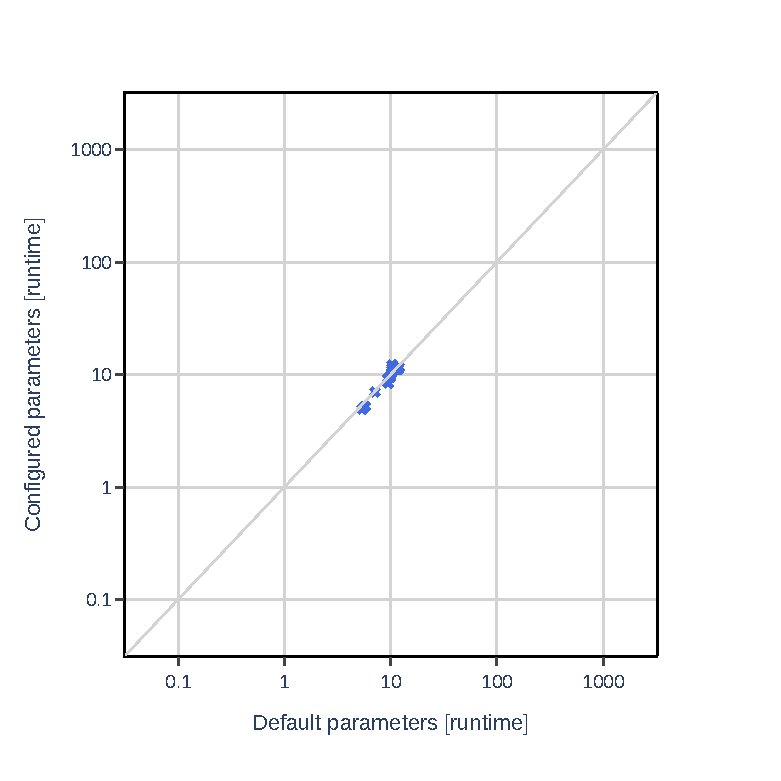
\includegraphics[width=0.6\textwidth]{data_SCIP_configured_vs_default_on_Europe_3h_year}
% \includegraphics[width=0.8\textwidth]{fittedModels}
\par\end{centering}

\caption{Empirical comparison between the SCIP (configured) and SCIP (default) on the training set of Europe\textunderscore 3h\textunderscore year.}\label{fig:configured_vs_default_train}
\end{figure}

%\ifruntime

Table \ref{tbl:timeouts_train} shows on how many instances the SCIP (configured) and SCIP (default) timed out (did not solve the instance within the cutoff time of 60 seconds) on the training set of Europe\textunderscore 3h\textunderscore year, as well as on how many instances both timed out.

    \begin{table}[htbp]
        \centering
            \begin{tabular}{ccc}
                configured & default & overlap \\ \hline
                0 & 0 & 0
            \end{tabular}
            \caption{Number of time-outs for SCIP (configured), SCIP (default), and for how many instances both timed out on the training set of Europe\textunderscore 3h\textunderscore year.}
        \label{tbl:timeouts_train}
    \end{table}

%\fi % End ifruntime

\iftest
    \section{Comparison between Configured Version and Default Version on the Testing Instance Set}

    After specifying the optimised configuration, \emph{Sparkle} ran the configured version of SCIP and the default version of SCIP on the testing instance set. During this phase, each version performed one run per instance with a cutoff time of 60 seconds. The results are reported as follows.

    \begin{itemize}
        \item \textbf{SCIP (configured)}, runtime: @@optimisedConfigurationTestingPerformance@@
        \item \textbf{SCIP (default)}, runtime: @@defaultConfigurationTestingPerformance@@
    \end{itemize}

    The empirical comparison between the SCIP (configured) and SCIP (default) on the testing set of @@instanceSetTest@@ is presented in Figure \ref{fig:configured_vs_default_test}.

    \begin{figure}[htbp]
        \noindent
        \begin{centering}
            @@figure-configured-vs-default-test@@
            \par
        \end{centering}

       \caption{Empirical comparison between the SCIP (configured) and SCIP (default) on the testing set of @@instanceSetTest@@.}\label{fig:configured_vs_default_test}
    \end{figure}

    %\ifruntime

        Table \ref{tbl:timeouts_test} shows on how many instances the SCIP (configured) and SCIP (default) timed out (did not solve the instance within the cutoff time of 60 seconds) on the testing set of @@instanceSetTest@@, as well as on how many instances both timed out.

        \begin{table}[htbp]
            \begin{center}
                \begin{tabular}{ccc}
                    configured & default & overlap \\ \hline
                    @@timeoutsTestConfigured@@ & @@timeoutsTestDefault@@ & @@timeoutsTestOverlap@@
                \end{tabular}
            \end{center}
            \caption{Number of time-outs for SCIP (configured), SCIP (default), and for how many instances both timed out on the testing set of @@instanceSetTest@@.}
            \label{tbl:timeouts_test}
        \end{table}

    %\fi % End ifruntime

\fi % End iftest

\ifablation
    \section{Parameter importance via Ablation}

    Ablation analysis~\cite{FawcettHoos16} is performed from the SCIP (default) to SCIP (configured) to see which parameter changes between them contribute most to the improved performance.
    \iftest
    The ablation path uses the training set Europe\textunderscore 3h\textunderscore year and validation is perform on the test set @@instanceSetTest@@.
    \else
    The ablation path is constructed and validated with the training set Europe\textunderscore 3h\textunderscore year.
    \fi
    The set of parameters that differ in the two configurations will form the ablation path.
    Starting from the default configuration, the path is computed by performing a sequence of rounds.
    In a round, each available parameter is flipped in the configuration and is validated on its performance.
    The flipped parameter with the best performance in that round, is added to the configuration and the next round starts with the remaining parameters.
    This repeats until all parameters are flipped, which is the best found configuration.
    The analysis resulted in the ablation path presented in Table~\ref{table:ablationpath}.


    \begin{table}[htbp]
        \caption{Ablation path from SCIP (default) to SCIP (configured) where parameters with higher importance are ranked higher.}
        \label{table:ablationpath}
        \begin{center}
        \footnotesize
            \begin{tabular}{rp{0.25\linewidth}rrr}\end{tabular}
        \end{center}
    \end{table}

\fi % End ablation

\bibliographystyle{plain}
\bibliography{/rwthfs/rz/cluster/home/vx475510/miniforge3/envs/sparkle/lib/python3.10/site-packages/sparkle/Components/Sparkle-latex-source/SparkleReport.bib}

\end{document}
